\documentclass[%
	%draft
	]{ijsra}
\def\IJSRAidentifier{\currfilebase} %<---- don’t change this!
%-------Title | Email | Keywords | Abstract-------------
\def\shorttitle{Study of Attitudes}
\def\maintitle{Study of Attitudes to Health and Religion in Medieval England}
\def\cmail{alba.menendez@outlook.com}
\def\keywords{History, Archaeology, Medieval, Hospitals, Religion, York, London}
%\def\keywordname{}%<--- redefine the name “Keywords“ in needed language
\def\abstract{The present paper analyses the evolution of attitudes towards health and religion within medieval hospitals in England through three case studies: St Leonard’s Hospital in York, and St Bartholomew’s and St Mary Spital in London. Medieval hospitals were religious institutions associated with a church, in which inmates, or cremetts, were nursed by members of the clergy, mostly nuns. Nursing relied upon a spiritual perspective based on worship and prayers; it was not until later periods that a scientific medical approach was introduced. In addition, these institutions cared for orphan children and the elderly, corrodians, as well as feeding the poor, the alms. This study provides a holistic picture of medieval hospitals in England, taking an interdisciplinary approach. It combines documentary evidence provided by historical sources on, for example, the economy of medieval hospitals, with archaeological evidence on the health and living conditions of the individuals inhabiting these institutions.}
%--------Author’s names------------
\def\authorone{Alba Menéndez Pereda}
%-------Biographical information-------------
\def\bioone{Alba Menéndez Pereda is an MPhil Archaeology student, specialising in Archaeology of the Americas, at the Division of Archaeology at the University of Cambridge.
After simultaneously obtaining the International Baccalaureate diploma and the Spanish Bachillerato in Madrid, she moved to England in 2013 to pursue her undergraduate studies at the University of Durham.  Alba graduated with a BA (First Class) in Archaeology and Ancient Civilisations in July 2016.

%Her research interests focus on the investigation of interactions between people with different ethnographical backgrounds, through the analysis of material culture. Led by this interest, Alba investigated, for her Undergraduate Dissertation, the impact that the interaction between the local Christian population and the incoming Islamic groups had on the Medieval (711--1492) glass industry in Spain. For her MPhil Thesis, Alba is planning on researching the cultural exchange carried out between the native population and the Spanish incomers who settled in Central and South America.
After finishing her Master’s, Alba hopes to be able to gain fieldwork experience outside Europe (for the time given she has collaborated in archaeological projects covering different periods in England, Italy and Spain), before pursuing a PhD programme.}
%------University/Institution--------------
\def\affilone{University of Cambridge}

\begin{filecontents}{\IJSRAidentifier.bib}
@book{Biller_2001,
	editor = {Biller, P. and Ziegler, J.},
	title = {Religion and medicine in the Middle Ages},
	date = {2001},
	series = {York Studies in Medieval Theology},
	number = {III},
	publisher = {The University of York},
	location = {Woodbridge},
}

@book{Bowers_2007,
	editor = {Bowers, B.S.},
	title = {The Medieval Hospital and Medical Practice},
	date = {2007},
	series = {AVISTA Studies in the History of Medieval Technology, Science and Art},
	volume = {3},
	publisher = {Ashgate},
	location = {Aldershot},
}

@book{Brodman_2009,
	author = {Brodman, J.},
	title = {Charity and religion in Medieval Europe},
	date = {2009},
	publisher = {The Catholic University of America Press},
	location = {Washington D.C.},
}

@book{Clay_1966,
	author = {Clay, R.M.},
	title = {The Mediaeval Hospitals of England},
	date = {1966},
	publisher = {Routledge},
	location = {London},
}

@misc{Cullum_1991,
	author = {Cullum, P.H.},
	title = {Cremetts and corrodies: care of the poor and the sick at St Leonard’s Hospital, York in the Middle Ages},
	series = {Borthwick Papers},
	date = {1991},
	publisher = {University of York},
	location = {York},
	number = {179},
}

@incollection{Cullum_1999,
	author = {Cullum, P.H.},
	editor = {Smith, D.M.},
	title = {St Leonard’s Hospital, York, in 1287},
	booktitle = {The Church in Medieval York. Records edited in honour of Professor Barrie Dobson},
	date = {1999},
	pages = {17--28},
	publisher = {University of York},
	location = {York},
}

@book{Dainton_1961,
	author = {Dainton, C.},
	title = {The Mediaeval Hospitals of England},
	date = {1961},
	publisher = {Museum Press Limited},
	location = {London},
}

@book{Dean_2008,
	author = {Dean, G.},
	title = {Medieval York},
	date = {2008},
	publisher = {The History Press},
	location = {Stroud},
}

@incollection{Egan_2007,
	author = {Egan, G.},
	editor = {B.S.},
	title = {Material culture of care for the sick: some excavated evidence from English medieval Hospitals and other sites},
	booktitle = {The Medieval hospital and Medieval practice},
	date = {2007},
	pages = {65--76},
	publisher = {Ashgate},
	location = {Aldershot},
}

@book{Goldberg_1992,
	author = {Goldberg, P.J.P.},
	title = {Women, work and life cycle in a Medieval economy. Women in York and Yorkshire, c. 1300-1520},
	date = {1992},
	publisher = {Claredon Press},
	location = {Oxford},
}

@book{Henderson_2006,
	author = {Henderson, J.},
	title = {The Renaissance Hospital. Healing the body and healing the soul},
	date = {2006},
	publisher = {Yale University Press},
	location = {London},
}

@online{Johnson_2014,
	author = {Johnson, A.},
	title = {A history of Archaeology Live! Year one: St. Leonard’s 2001},
	date = {2014},
	url = {https://archaeologylive.wordpress.com/2014/06/20/a-history-of-archaeology-live-year-one-st-leonards-2001},
	organization = {Archaeology Live!},
	urldate = {2015-04-20},
}

@book{Malcom_2014,
	author = {Malcom, G. and Sloane, B.},
	title = {Excavations at the priory of the Order of the Hospital of St John of Jerusalem, Clerkenwell, London},
	date = {2014},
	publisher = {Museum of London Archaeology Service},
	location = {London},
}

@book{Orme_1995,
	author = {Orme, N. and Webster, M.},
	title = {The English Hospital. 1070-1570},
	date = {1995},
	publisher = {Yale University Press},
	location = {London},
}

@online{Page_1974,
	author = {Page, W.},
	title = {Victoria County History},
	date = {1974},
	url = {http://www.british-history.ac.uk/vch/yorks/vol3/pp336-352},
	subtitle = {A history of the County of York. Volume 3},
	organization = {British History Online},
	urldate = {2015-04-20},
}

@book{Palliser_2014,
	author = {Palliser, D.M.},
	title = {Medieval York. 600-1540},
	date = {2014},
	publisher = {Oxford University Press},
	location = {Oxford},
}

@book{Phillpotts_1997,
	author = {Thomas, C. and Sloane, B. and Phillpotts, C.},
	title = {Excavations at the Priory and Hospital of St Mary Spital, London},
	date = {1997},
	publisher = {Museum of London Archaeology Service},
	location = {London},
}

@book{Raine_1955,
	author = {Raine, A.},
	title = {Mediaeval York. A topographical survey based on original sources},
	date = {1955},
	publisher = {John Murray},
	location = {London},
}

@book{Rawcliffe_1995,
	author = {Rawcliffe, C.},
	title = {The hospitals of Medieval Norwich. Studies in East Anglian History 2},
	date = {1995},
	publisher = {University of East Anglia},
	location = {Norwich},
}

@book{Rawcliffe_1999,
	author = {Rawcliffe, C.},
	title = {Medicine for the soul. The life, death and resurrection of an English Medieval Hospital. St Giles’s, Norwich, c. 1249-1550},
	date = {1999},
	publisher = {Sutton Publishing},
	location = {Stroud},
}

@book{Rawcliffe_2004,
	editor = {Rawcliffe, C. and Wilson, R.},
	title = {Medieval Norwich},
	date = {2004},
	publisher = {Hambledon},
	location = {London},
}

@book{Rider_2012,
	editor = {Rider, C.},
	title = {Magic and Religion in Medieval England},
	date = {2012},
	publisher = {Reaktion Books},
	location = {England},
}

@article{Rogers_2001,
	author = {Rogers, J. and Waldron, T.},
	title = {DISH and the Monastic Way of Life},
	journaltitle = {International Journal of Osteoarchaeology},
	year = {2001},
	volume = {11},
	number = {5},
	pages = {357--365},
}

@misc{Stell_1996,
	author = {Stell, P.},
	title = {Medical practice in Medieval York},
	series = {Borthwick Papers},
	date = {1991},
	publisher = {University of York},
	location = {York},
	number = {90},
}

@book{Thomas_2002,
	editor = {Thomas, C. },
	title = {The archaeology of medieval London},
	date = {2002},
	publisher = {Sutton Publishing},
	location = {Stroud},
}

@online{Unknown_1957,
	editor = {Sheppard, F.H.W.},
	title = {Survey of London: Volume 27, Spitalfields and Mile End New Town, pp.21-23},
	date = {1957},
	url = {http://www.british-history.ac.uk/survey-london/vol27/pp21-23},
	subtitle = {The Priory of St. Mary Spital},
	organization = {British History Online},
	urldate = {2016-08-16},
}

@article{Verlaan_2007,
	author = {Verlaan, J. and Oner, F. and Maat, G.},
	title = {Diffuse idiopathic skeletal hyperostosis in ancient clergymen},
	journaltitle = {European Spine Journal},
	date = {2007},
	volume = {16},
	number = {8},
	pages = {1129--1135},
}

@article{Waldron_1985,
	author = {Waldron, T.},
	title = {DISH at Merton Priory: evidence for a "new" occupational disease? },
	journaltitle = {British Medical Journal},
	date = {1985},
	volume = {291},
	pages = {1762--1763},
}

@article{Watson_2006,
	author = {Watson, S.},
	title = {The Origins of the English Hospital},
	journaltitle = {Transactions of the Royal Historical Society: Sixth Series},
	date = {2006},
	volume = {16},
	pages = {75--94},
}

@incollection{White_2007,
	author = {White, W.},
	editor = {Bowers, B.S.},
	title = {Excavations at St Mary Spital: burial of the “Sick Poore” of Medieval London, the evidence of illness and hospital treatment},
	booktitle = {The Medieval hospital and Medieval practice},
	date = {2007},
	pages = {59--64},
	publisher = {Ashgate},
	location = {Aldershot},
}

@online{YorkMuseumGardens_2016,
	title = {St Leonard’s Hospital},
	date = {2016},
	url = {http://www.yorkmuseumgardens.org.uk/about/st-leonards-hospital/},
	OPTorganization = {York Museum Gardens},
	OPTdate = {20},
	OPTmonth = {09},
	OPTyear = {2016},
}


\end{filecontents}
\renewcommand\AD{\xspace}
\begin{document}
\IJSRAopening%<---- don’t change this!
%-------
\lettrine{T}{here} have been many publications discussing medieval hospitals\footnote{Before the topic of medieval hospitals can be discussed, it is necessary to clarify that these institutions, which were already very numerous in England in the 13th century, did not function in the same way as modern-day hospitals. They were ecclesiastical rather than medical organisations that provided nursing care and religious relief for the sick and poor, as opposed to strictly medical treatment \parencite{Clay_1966}.} 
in the last fifty years, by both archaeologists and historians \parencites{Cullum_1991}{Phillpotts_1997}{Rawcliffe_1999}{White_2007}. 
Historians, who base their knowledge on written documentary evidence, have obtained vast amounts of information on the organisation of these institutions. Additionally, following analysis of material remains recovered at the hospitals, archaeologists have recovered information related to the everyday life of the hospitals’ inhabitants. Nevertheless, it is not always clear to scholars what exactly the activities of these early hospitals were, since most papers focus on specific case studies, or on leper houses, which have been more widely researched \parencite[76-78]{Watson_2006}. 
Some questions, such as how the development of medieval religious hospitals led into modern ideas of medical treatment and hospital care, remain uncertain.

Three case studies are considered here: St Leonard’s Hospital, York, believed to be the largest medieval hospital in northern England, and one of the wealthiest in the country; St Bartholomew’s Hospital, London, the oldest hospital in England to continuously provide care at its original site until modern times; and St Mary Spital, the largest institution of this type in London, and one of the best-excavated medieval hospitals. 
These three sites have been analysed using a combination of documentary and archaeological evidence, in order to obtain a comprehensive picture of how this type of religious institution operated. This analysis is used to develop an informed picture of how medicine was practiced at these English institutions, and how these practices evolved throughout the medieval period, eventually incorporating newly acquired scientific knowledge.


\IJSRAsection{St Leonard’s Hospital, York}
St Leonard’s Hospital at York (\cref{fig:Pereda-Figure01}) %XXX
 was one of the largest and wealthiest medieval hospitals in England, and it has been a major focus of research in historical investigations. However, no archaeological work was carried out at the site until the \nth{21} century. 
 At this time, excavation began in a limited area of what was known to be St Leonard’s Hospital infirmary.
 
\begin{wrapfigure}{O}{0.5\textwidth}  		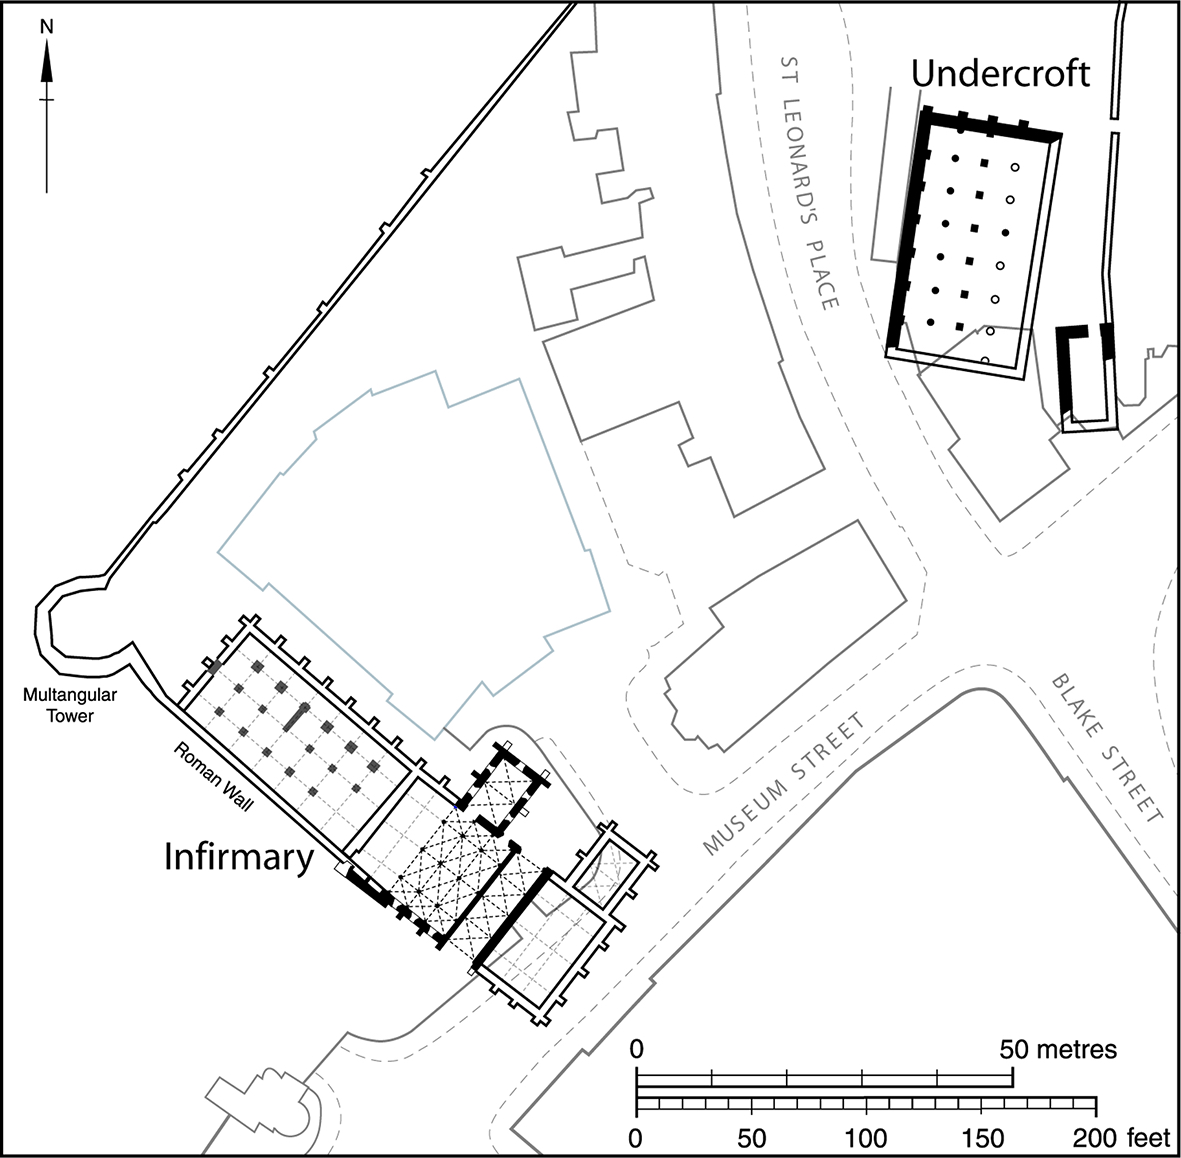
\includegraphics[width=\linewidth]{figures/Pereda-Figure01}
 		\caption{St Leonard’s Hospital plan.
    {\normalfont\scriptsize \\ Obtained from \textcite[100, fig. 37]{Dean_2008}.
              }}
 		\label{fig:Pereda-Figure01}
 	\end{wrapfigure}
 The hospital assisted permanent invalids, the chronically ill, and the acutely ill, in addition to the orphans who attended the attached grammar and singing school. Inmates were allowed to stay until they were recovered and capable of working. They were nursed by the sisters, but other than evidence for the purchase of medicines, not much is known about the medical treatments provided at St Leonard’s Hospital \parencites[5,12-15]{Cullum_1991}[21]{Dainton_1961}[97]{Dean_2008}[134]{Goldberg_1992}{Page_1974}[78,109]{Palliser_2014}.
 
 \IJSRAsubsection{History}
Documentary evidence establishes that St Leonard’s Hospital was founded ca.\,936 by King Athelstand, as the Hospital of St Peter, and was located on the western corner of the York Roman fortress. It received the royal privilege of “Petercorn”, though which it was granted corn from all the fields in the diocese. The hospital was re-founded as St Leonard’s Hospital in the \nth{11} century\AD on the orders of King Stephen, and survived until December \nth{1}, 1538, when the hospital was forced to surrender its properties to the Crown 
\parencite[288]{Palliser_2014}. This situation left the city of York lacking a hospital from the time of Henry VIII until the first half of the \nth{18} century\AD \parencite{YorkMuseumGardens_2016}.
\clearpage
\IJSRAsubsection{Hospital complex}
Archaeological excavation suggests that parts of earlier structures were incorporated in the foundations of the medieval hospital. Of the structures that composed St Leonard’s hospital, only a gate, the chapel, and the infirmary (with vaulted under croft) remain in situ. During excavation, part of the stone drain of the hospital was discovered, indicating the existence of a complex drainage system that took the sewage from the infirmary out of the hospital´s precinct \parencite{Johnson_2014}, which would have helped to maintain the hospital in a higher standard of cleanliness than the average domestic living space.
The Rule of 1295 establishes that St Leonard’s was organised around two courtyards. One of them was for the church and the brothers, and the other courtyard was dedicated to the actual hospital. The hospital precinct could be accessed through two doors, one of which was located at the infirmary and the other of which, known as Watergate, was located on Blake Street, where bread, meat and ale were provided weekly to the alms \parencites[8-9,28-29]{Cullum_1991}[17]{Cullum_1999}{Johnson_2014}[151]{Palliser_2014}[116]{Raine_1955}[314]{Rawcliffe_2004}.

Extensive building activity occurred during the \nth{13} century\AD, including the enlargement of the infirmary. At this time, St Leonard’s was known to have had a church, school, orphanage, hospital, Master’s house, residences for the brothers and sisters, a tannery, smithy, brew house, horse mill, carpenter´s shop, and stables 
\parencites[99]{Dean_2008}[116]{Raine_1955}. This indicates that St Leonard’s Hospital was almost completely self-sufficient. These production centres were not only employed to supply the hospital; St Leonard’s also participated in a range of both commercial and charitable activities, exchanging the goods produced at the hospital and providing for the poor.

 \IJSRAsubsection{Inhabitants}
By the late \nth{13} century\AD, the hospital started accepting lepers, causing the number of inmates to peak at over \num{220} individuals, as well as 23 orphans \parencites[6,10]{Cullum_1991}[151]{Palliser_2014}. The hospital could not have maintained this figure overtime, due to a decrease in its financial income. 
Moreover, in the \nth{14} century\AD, due to its precarious economic state, the hospital started accepting the entrance of a large number of corrodians. They were old, wealthy individuals, who paid in cash or in kind to spend the rest of their lives in the hospital, no matter their health conditions. 

However, the expense corrodians incurred is still likely to have been greater than the income they brought to the hospital \parencites[235]{Brodman_2009}[6]{Cullum_1991}. This practice can be interpreted as an early sign of hospitals as providers of remunerated services, rather than just charitable institutions, as well as the medieval precursor of homes for the elderly.
Archaeological evidence
Material remains recovered during excavations at the site include animal bones, glass artefacts, pottery, and a bronze seal ring \parencite{Johnson_2014}. These can be used to obtain information about the daily life of the hospital’s inhabitants. Their diet was known to be more varied and of a better quality than the average members of York’s population, which would have contributed to the inmates’ recovery. 
The everyday menu at the hospital included beef, mutton, pork, beans, honey, bread, ale, and pottage, but lacked fresh fruits and vegetables, which were not widely consumed in medieval society \parencites[16-17]{Cullum_1991}[19]{Cullum_1999}. 
Evidence for the hospital’s wealth can be observed in the infirmary decoration, which included decorated ridge tiles, glazed floor tiles and decorated window glass \parencite[101]{Dean_2008}. 
\IJSRAseparator\clearpage

\IJSRAsection{St Bartholomew’s Hospital, London}%
The site of the medieval hospital of St Bartholomew in London has not been excavated completely, as it is located beneath the modern St Bartholomew’s Hospital. However, rescue archaeology has been carried out and some material has been recovered.
\begin{figure}[!b]
		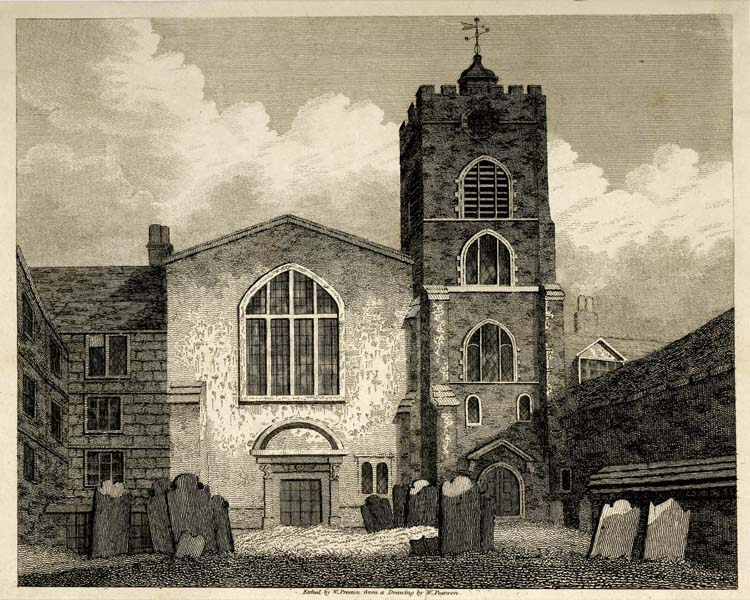
\includegraphics[width=.5\linewidth]{figures/Pereda-Figure02}
		\caption{Engraving from 1810 depicting St Bartholomew’s the Great Church, the only surviving element of the original medieval hospital located at the site of the modern St Bartholomew’s Hospital. Artefact ID No.: A19933. Retrieved 20 August 2016.
		{\normalfont\scriptsize \\ \copyright\ Museum of London}}
		\label{fig:Pereda-Figure02}
\end{figure}

\IJSRAsubsection{History}
In situations such as this, the work carried out by historians is fundamental to shed light on the activities of the hospital. St Bartholomew’s Hospital (\cref{fig:Pereda-Figure02}) %XXX
was originally founded ca.\,1123 by the adventurer Rahere, with the aid of the Bishop of London, and was re-founded in the time of Henry\,VIII. During this period, the hospital’s income relied on donations collected by a representative sent into towns on behalf of the hospital \parencite[19,42]{Dainton_1961}. 
The importance of this hospital lies in the fact that it is the oldest hospital in England which has continued caring for the sick at its original site since its foundation \parencite[35]{Dainton_1961}. 
Additionally, it was one of the first hospitals in the country to provide education for children \parencite[21]{Rawcliffe_1999}. 


\IJSRAsubsection{Treatments employed}
In the \nth{14} century\AD, a group of four Augustinian nuns assisted the inmates while living communally within the hospital’s precinct. As was usual in medieval times, the care they provided for the sick was based on spiritual relief and religious well-being, delivered through religious sacraments and participation in religious services. 
Nevertheless, evidence for some kind of medical treatments practiced at the hospital can be found in, for example, Breviarium Bartholomei, written by the priest and medical writer, John Mirfield \parencite[36-37]{Dainton_1961}. 
This occasionally included the employment of charms and other magical features, such the selection of specific days of the month to perform bloodletting \parencite[35-36]{Rider_2012}. 
It was not until after the hospital’s re-foundation, which took place in 1546, that staff with actual medical knowledge were employed. The hospital staff included surgeons, physicians and barbers, in addition to the apothecary who prepared the medicines prescribed by the physicians \parencite[38-39]{Dainton_1961}. This demonstrates a change within hospital treatment, as well as societal attitudes.  
The continuous running of St Bartholomew’s exhibits in a clear way the transformation of former religious medical care into an expert scientific discipline, marked at this site by the advances made on the research of the circulatory system and modern surgery between the \nth{17} and \nth{18} centuries.
\IJSRAseparator

\IJSRAsection{St Mary Spital, London}
The Priory and Hospital of the Blessed Virgin Mary without Bishopsgate (\cref{fig:Pereda-Figure03}), %XXX FIG
known as St Mary Spital, was located in north-east London, and grew to be the largest Medieval hospital in London \parencite[60]{Bowers_2007}. It has been progressively surveyed over the last century, and is therefore one of the best-excavated medieval hospitals. 
\begin{figure}[!b]
		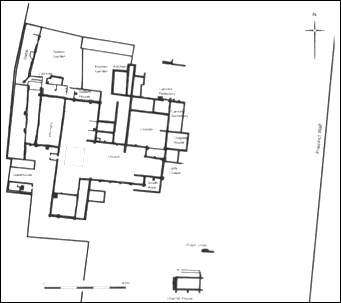
\includegraphics[width=.5\linewidth]{figures/Pereda-Figure03}
		\caption{St Mary Spital plan.
		        {\normalfont\scriptsize \\ Obtained from \textcite[98, fig. 37]{Thomas_2002}.
		                  }}
		\label{fig:Pereda-Figure03}
	\end{figure}
\IJSRAsubsection{History}
St Mary Spital was founded at the beginning of the \nth{12} century\AD by a group of wealthy London merchants, and dissolved under Henry VIII in 1539, leading to the development of the former parish of Spitalfields. Initially, the hospital only assisted the poor and the sick, but through time it also cared for the well-being of pilgrims, migrants, pregnant women, children under the age of seven, and the elderly \parencites[26]{Phillpotts_1997}[48-49]{Thomas_2002}{Unknown_1957}[60-61]{White_2007}.

\IJSRAsubsection{Hospital complex}
The original hospital consisted of a small rectangular structure, most of which was dedicated to housing 13 inmates, and the rest of which was a chapel. This spatial organisation enabled the inmates to see the altar from their beds, which was thought to be indispensable for their recovery \parencites[91]{Phillpotts_1997}[98]{Thomas_2002}.
The second infirmary, dating to the hospital’s re-foundation, was a T-shaped structure divided by a church lying in the centre, forming two separate infirmaries with different entrances, between which the sexes were divided. The hospital included 60 beds, 30 for men and 30 for women, placed against the walls and separated by a central aisle \parencites[37]{Phillpotts_1997}[99]{Thomas_2002}. 
In the \nth{14} century\AD, the old infirmary became a chapel, and a new two-storey structure was built to house the new infirmary. Here, the sexes were likely to have been separated over the two floors. This structure held 90 shared beds and, therefore, possibly up to 180 inmates.
Excavations have revealed the presence of a hearth in the northeast corner of the ground floor, where the sisters might have warmed up food and/or prepared herbal remedies. Soon after its construction, the infirmary was expanded due to the increasing number of individuals entering the hospital \parencites[47]{Phillpotts_1997}[99]{Thomas_2002}[59]{White_2007}. 
After the \nth{14} century\AD, timber structures were built to house the incoming corrodians \parencite[104,152]{Thomas_2002}.

To the north of the infirmary was the refectory, where the brothers ate while listening to passages from the Bible, as was also the case at St Leonard’s Hospital. 
To the north-west was the kitchen \parencites[51]{Phillpotts_1997}[100]{Thomas_2002}; 
towards the west of the infirmary was a cemetery in which the deceased were buried in nine rows, each row with a maximum of 25 burials \parencite[59]{White_2007}; and the brothers’ dormitory was located towards the east, on a first-floor level, with the chapter house and storage area underneath. The southern area of the precinct was used for agricultural purposes and to house animals.

The sisters lived originally in a timber house with mortar floor. Their low status can be inferred from the fact that they were the last members to receive a stone structure in which to live, a conclusion that agrees with the documentary evidence \parencites[36]{Phillpotts_1997}[51]{Rawcliffe_1999}[151]{Thomas_2002}.
St Mary Spital, like St Leonard’s, had its own water supply and drains that ran the waste from the kitchens and the latrines out of the precinct of the hospital \parencite[151]{Thomas_2002}. 
\IJSRAseparator

\IJSRAsection{Archaeological evidence}
Through excavation, a set of keys was found in the \nth{13} century infirmary. They might have been used to open lockers owned by the inmates \parencite[99]{Thomas_2002}. In a pit outside the infirmary, a group of 18~wooden bowls and plates, ceramic vessels, and a pair of leather boots were found well preserved, due to waterlogged conditions. The bowls (\cref{fig:Pereda-Figure04}), %XXX FIG
which have different marks that might have indicated their users, were probably used to feed the sick \parencites[68]{Egan_2007}[99]{Thomas_2002}. 
Nearby, a large number of animal bones were uncovered and used to obtain information about the diet provided at the hospital, which included high proportions of fish and meat \parencite[59,113-114]{Phillpotts_1997}.
In another pit, seven gold coins issued under the kingdom of Henry\,VIII were discovered. These coins were thought to protect against evil through the impressed image of the archangel St Michael and the inscription in Latin: \enquote{Through your cross, save us, Christ, Redeemer.}  \parencite[70]{Egan_2007}. 

These are a clear example of magical charms employed to prevent and treat sickness within Christian contexts.
At least \num{10500} individuals were buried in the hospital’s cemetery. These skeletal remains provide insight into the kinds of patients for which the hospital cared.  Burials are varied; alongside simple interments lacking coffins and not always aligned in the east-west orientation, there were also high-status individuals buried in lead or stone coffins. Five tombs containing individuals identified as priests included a pewter calyx and a paten for sacramental duties after resurrection. 

An interesting feature is the presence of mass burials in which the deceased are facing downwards, which might evidence a plague that spread in London before the Black Death \parencites[61]{Bowers_2007}[252]{Brodman_2009}[73]{Egan_2007}[101]{Thomas_2002}[61]{White_2007}.
A large number of the individuals interred in the cemetery present skeletal pathologies, elucidating diseases from which the citizens of medieval London may have suffered. For example, several individuals presented lesions consistent with diffuse idiopathic skeletal hyperostosis (DISH); a medical condition caused by a diet rich in animal fats and expressed through the fusion of vertebrae and the overgrowth of bone. This disease has been associated particularly with male members of increasing age within the higher clergy during the Middle Ages, who were a minority able to access plenty of food supplies. 

They may also have suffered from obesity and diabetes mellitus, risk factors to developing DISH
\parencites[361-362]{Rogers_2001}{Verlaan_2007}[1763]{Waldron_1985}[62]{White_2007}.
Evidence of surgical treatments performed at the hospital can also be identified in the skeletal remains. 

Skeletal trauma shows signs of healing, suggesting that individuals were surviving procedures such as trepanations and lower limb amputations \parencite[63-64]{White_2007}. This change within medical practice, already appreciated at the other sites, might have been a response to the society’s changing needs.

Sheets of metal plates were found at three burials containing textile remains in the inner side, similar to the finds recovered at Merton Priory, London, and Gilbertine Priory of St Andrew, York. These metal plates might have been used to protect long-term bandages, which could have contained medical preparations \parencite[70-71]{Bowers_2007}. 
Besides this evidence of sophisticated medical practice, other interesting artefacts proving a religious perspective on health and death were also found at some burials of the Mary Spital cemetery. They include five papal lead seals, bullae, dating back to the \nth{14} century\AD. They have the name of Pope Urban\,VI inscribed upon them, and used to be attached to documents that proved that the deceased have had their sins pardoned \parencites[69]{Phillpotts_1997}[70,72]{White_2007}.

\begin{figure}[!h]
		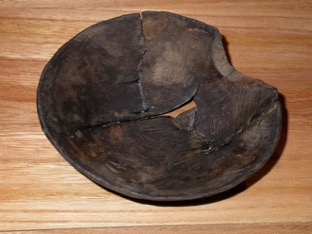
\includegraphics[width=.5\linewidth]{figures/Pereda-Figure04}
		\caption{One of the wooden bowls recovered from St Mary Spital. They contained scratched marks and might have been used to feed the sick.
		{\normalfont\scriptsize \\ \copyright\ Museum of London; Image obtained from Museum of London. Artefact ID No.: NRF88[1286]<611>. Retrieved 20 August 2016.}}
	\label{fig:Pereda-Figure04}
   \end{figure}

\IJSRAseparator
\IJSRAsection{Discussion and Conclusion}
Only through the combination of all sources of evidence (historical documents and material remains) available, can a complete and comprehensible picture of past societies be obtained. When material evidence cannot be accessed, such as in the case of St Bartholomew’s Hospital, or has been lost, documents can fill the gaps. Conversely, archaeological remains can support or challenge what is written in the documentary evidence. Investigations of medieval hospitals need to be approached from historical and archaeological perspectives in order to allow researchers to provide the most accurate conclusions possible. 

As indicated by the documentary and material evidence exhibited for the three case studies investigated in the present paper, the complex of medieval hospitals was similar to the monastic design. They usually consisted of a chapel, cloisters, refectory, infirmary, and gardens where agricultural activities for commercial and self-provisioning purposes, and human burials took place. 

The evolution of hospital complexes is not easily understood, due to their constant development and refurbishment, which in cases such as St Mary Spital was due to the continuous need for larger structures to house the increasing numbers of incoming inmates \parencites[69,117-118]{Henderson_2006}[27]{Malcom_2014}[41,43]{Orme_1995}[35]{Rawcliffe_1999}.
Medieval hospitals based their income on the donations made by wealthy individuals who wanted their charitable acts to be considered in purgatory. However, due to a decrease in income, from the \nth{14} century\AD onwards, hospitals began to accept more corrodians than cremetts \parencites[69]{Dean_2008}[207]{Malcom_2014}. 

Hospitals originally operated as religious institutions, worship being their primary function. This is evidenced by the central position that chapels occupied within the infirmaries at St Mary Spital, St Bartholomew’s and St Leonard’s, and the obligation for the sick to attend their services. Brothers lived in the hospitals accompanied by sisters who assisted the inmates (old, wealthy individuals, the poor, the sick, orphans, and pregnant women), and the lay workers who behaved to some extent as religious individuals, attending services and living in a community in which men were separated from women, as has been exhibited in the cases of St Leonard’s and St Mary Spital. 

Archaeological excavations provide more material evidence related to the spiritual well-being of the inmates than to medical treatments; evidence for the latter is rare, and consists mainly of evidence for interventions on skeletal remains, such as those at St Mary Spital, as no medical instrument has been clearly identified \parencite[65,76]{Bowers_2007}. 
It is necessary to take into account that medieval medical implements are likely to have greatly differed from modern ones and might not be easily recognisable as such. Additionally, there might be some level of predisposition from researchers to interpret finds recovered at medieval hospitals as religious rather than scientific, due to the ecclesiastical nature of the sites. 
Religious relief, the reconciliation of a soul cleansed of sins with God, was the way to cure or alleviate physical pains, which were understood as punishments from God \parencites[12-13,96]{Biller_2001}[42-43]{Rawcliffe_1995}. 

Besides treating the inmates’ spiritual health, the treatments carried out by nuns consisted of cleaning, feeding, clothing and housing the patients; acts likely to have contributed to the inmates’ physical recovery, even if divine intervention alone was credited. Material evidence from St Mary Spital and St Leonard’s indicates that the diet consumed by the people living at medieval hospitals was varied, and better than regular citizens’ food. Some of this food was produced on the grounds of the hospital, while other products were obtained through donations \parencites[76]{Egan_2007}[208]{Malcom_2014}.

Nevertheless, the epidemic diseases that spread during the \nth{14} century\AD provoked a stronger engagement of individuals with medical knowledge indicated by the survival of medical manuscripts, 

such as Breviarium Bartholomei from St Bartholomew’s Hospital \parencite[6,16-22]{Stell_1996}. 
In conclusion, early medieval hospitals provided a broader range of services than their modern counterparts and might be better regarded as charitable institutions, rather than strict medical centres in their modern significance. Nevertheless, from the \nth{14} century\AD onwards, advances in medicine were developed, and were slowly incorporated into these religious hospitals, until scientific treatments eventually replaced the exclusively religious care that was originally central to medieval hospitals. 

\iffalse
Illustrations
Figure 1. St Leonard’s Hospital plan. Obtained from Dean, 2008: 100, figure 37.
Figure 2. Engraving from 1810 depicting St Bartholomew’s the Great Church, the only surviving element of the original medieval hospital located at the site of the modern St Bartholomew’s Hospital. Artefact ID No.: A19933. ©Museum of London. Retrieved 20 August 2016.
Figure 3. St Mary Spital plan. Obtained from Thomas, 2002: 98, figure 37.
Figure 4. One of the wooden bowls recovered from St Mary Spital. They contained scratched marks and might have been used to feed the sick. Image obtained from Museum of London. Artefact ID No.: NRF88[1286]<611>. ©Museum of London. Retrieved 20 August 2016.
\fi
\IJSRAclosing%<---- don’t change this!
\end{document}